\section{Лекция 1 24.02.25. Численные методы решения нелинейных уравнений и систем}
\subsection{Постановка задачи}
Пусть $\mathbf{x} = \begin{pmatrix} 
x_1    \\ 
x_2    \\ 
\vdots \\ 
x_n    
\end{pmatrix} \in \mathbb{R}^n, F \in C(\mathbb{R}^n).
$
Дано уравнение:
\begin{equation}
F(\mathbf{x}) = 0. 
\end{equation}
Требуется найти вектор $\mathbf{x^*} \in \mathbb{R}^n$ такой, что $F(\mathbf{x^*}) = 0$.
\subsection{Проблемы в вычислительном контексте}
\subsubsection{Устойчивость}
Пусть мы имеем уравнение
\[
x^2 + px + q = 0.
\]
Известно, что если $p^2 = 4q$,
то уравнение имеет единственное решение.
Если в вычислительном эксперименте вместо $p$ и $q$ получить $p^*$ и $q^*$ соответственно, то могут появиться ложные решения или пропасть настоящие.
\subsubsection{Построение $\varepsilon$-решения}
\paragraph{Определение ($\varepsilon$-решение):} Вектор $\mathbf{x^*}$, удовлетворяющий неравенству
$
\|F(\mathbf{x^*})\| < \varepsilon,
$
называется $\varepsilon$-решением уравнения (1).

Откуда брать $\varepsilon$? Универсальной процедуры нет. Нужно брать значение, соответствующее прогрешности, исходя из природы задачи.
\paragraph{Пример:} 
$\varepsilon = 1,6 \cdot 10^{-19}$ Кл. (уравнение электронного заряда).
\subsubsection{Недостаточность $\varepsilon$-решения}
\begin{center}
    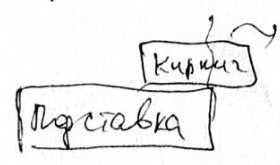
\includegraphics[width=5.2cm]{../figures/lection_1/figure_1.png}
\end{center}
Кирпич, стоящий на подставке --- система в состоянии неустойчивого равновесия. Нас интересует поиск момента фазового перехода (момента, когда кирпич упадёт), точно так же как для плавления, кристаллизации, таяния и других примеров систем. В теории динамических систем это называют точкой бифуркации. Если мы найдём $\varepsilon$-решение, оно не подойдёт, так как нужно, чтобы произошёл <<переход через ноль>>, иначе решение не будет представлять ценности. Может быть найдена не одна точка $x^*$, а интервал.
\paragraph{Определение (точка перехода через ноль в одномерном случае):} $x^*$ --- точка перехода через ноль для $f\in C(\mathbb{R})$, если $\forall \varepsilon > 0 \  f(x^*-\varepsilon)f(x^*+\varepsilon) < 0$.
\subsection{Переход через ноль в многомерном случае}
Пусть $M \subset \mathbb{R}^n$.
\paragraph{Определение (векторное поле):} $\varphi:M\rightarrow\mathbb{R}^n$ --- векторное поле.
